% Common notations, theorems and procedures

\section{Notations\label{section:notations}}


The following notations will be used throughout this document:
\begin{itemize}

\item  $+$, $-$ and  $\times$ denote the usual
mathematical operations.

\item $\oplus$, $\ominus$ and $\otimes$ denote the
corresponding floating-point operations in IEEE-754 double precision,
in the IEEE-754 \emph{round to nearest} mode.

\item $\round(x)$, $\roundup(x)$ and $\rounddown(x)$ denote the value
  of $x$ rounded to the nearest, resp. rounded up and down.
  
\item $\epsilon$ (usually with some index) denotes a relative error,
  $\delta$ denotes an absolute error. Upper bounds on the absolute value of these errors
  will be denoted $\maxeps$ and $\maxdelta$.

\item $\maxeps_{-k}$ -- with a negative index -- represents an error $e$ such that $|e| \leq 2^{-k}$.
  
\item For a floating-point number $x$, the value of the least
  significant bit of its mantissa is classically denoted $\ulp(x)$.

\end{itemize}




\section{Common C procedures for double-precision numbers\label{section:commonCdouble}}

\subsection{Sterbenz Lemma \label{sec:sterbenz}}

\begin{theorem}[Sterbenz Lemma~\cite{Ste74,Gol91}]
\label{sterbenz}
If $x$ and $y$ are floating-point numbers, and if ${y}/{2} \leq x \leq
2y$ then $x\ominus y$ is computed exactly, without any rounding error.
\end{theorem}


\subsection{Double-precision numbers in memory\label{section:memory}}

A double precision floating-point number uses $64$ bits. The unit of
memory in most current architectures is a 32-bit word. The order in
which the two $32$ bits words of a double are stored in memory depends
on the architecture. An architecture is said \emph{Little Endian} if
the lower part of the number is stored in memory at the smallest
address; It is the case of the x86 processors. Conversely, an
architecture with the high part of the number stored in memory at the
smallest address is said \emph{Big Endian}; It is the case of the
PowerPC processors.

In \crlibm, we extract the higher and lower parts of a double by using
an union in memory: the type \texttt{db\_number}. The following code
extracts the upper and lower part from a double precision number $x$.

\begin{lstlisting}[label={chap0:lst:endian},
  caption={Extract upper and lower part of a double precision number $x$},firstnumber=1]
  /* HI and LO are defined automatically by autoconf/automake.  */

db_number xx;
int x_hi, x_lo;
xx.d = x;
x_hi = xx.i[HI]
x_lo = xx.i[LO]
\end{lstlisting}




\subsection{Conversion from floating-point to integer \label{sec:double2int}}

\begin{theorem}[Conversion floating-point to integer]
  The following algorithm, taken from \cite{AMDoptim2001}, converts a
  double-precision floating-point number $d$ into a 32-bit
  integer $i$ with rounding to nearest mode.

  It works for all the doubles whose nearest integer fits on a 32-bit machine signed integer.

\begin{lstlisting}[label={chap0:lst:conversion2},caption={Conversion from FP to int},firstnumber=1]
#define DOUBLE2INT(i, d)   \
  {double t=(d+6755399441055744.0); i=LO(t);}
\end{lstlisting}
\end{theorem}

This algorithm adds the constant $2^{52}+2^{51}$ to the floating-point
number to put the integer part of $x$, in the lower part of the
floating-point number.  We use $2^{52}+2^{51}$ and not $2^{52}$,
because the value $2^{51}$ is used to contain possible carry
propagations with negative numbers.


\subsection{Conversion from floating-point to 64-bit integer \label{sec:double2longint}}

\begin{theorem}[Conversion floating-point to a long long integer]
  The following algorithm, is derived from the previous.

  It works for any double whose nearest integer is smaller than $2^{51} -1$.

\begin{lstlisting}[label={chap0:lst:conversion3},caption={Conversion from FP to long long int},firstnumber=1]
#define DOUBLE2LONGINT(i, d)                                      \
  {                                                               \
    db_number t;                                                  \
    t.d = (d+6755399441055744.0);                                 \
    if (d >= 0) /* sign extend */                                 \
      i = t.l & 0x0007FFFFFFFFFFFFLL;                             \
    else                                                          \
      i = (t.l & 0x0007FFFFFFFFFFFFLL) |  (0xFFF8000000000000LL); \
  }
\end{lstlisting}

\end{theorem}




\subsection{Methods to raise IEEE-754 flags}

The IEEE standard imposes, in certain cases, to raise flags and/or
exceptions for the $4$ operators ($+$, $\times$, $\div$, $\sqrt{~}$).
Therefore, it is legitimate to require the same for elementary
functions.

In ANSI-C99, the following instructions raise exceptions and
flags:

\begin{itemize}
\item {\bf underflow} : the multiplication $\pm smallest \times smallest$ where $smallest$ correspond to the smallest subnormal number,
\item {\bf overflow} : the multiplication  $\pm largest \times largest$ where $largest$ correspond to the largest normalized number,
\item {\bf division by zero} : the division $\pm 1.0/0.0$,
\item {\bf inexact} : the addition $(x + smallest) - smallest$ where $x$ is the result and  $smallest$ the smallest subnormal number,
\item {\bf invalid} : the division $\pm 0.0/0.0$.
\end{itemize}








\section{Common C procedures for double-double arithmetic\label{section:commonCdoubledouble}}
Hardware operators are usualy limited to double precision. To perform
operations with more precision, then software solutions need to be
used. One among them is to represent a floating point number as the
sum of two non-overlapping floating-point numbers (or
\emph{double-double} numbers). 

The algorithms are given as plain C functions, but it may be
preferable, for performance issue, to implement them as macros, as in
\texttt{libultim}.  The code offers both versions,
selected by the \texttt{DEKKER\_AS\_FUNCTIONS} constant which is set
by default to 1 (functions).

A more recent proof is available in \cite{Lauter2005LIP:tripledouble}.

\subsection{Exact sum algorithm {Add12}}

This algorithm is also known as the Fast2Sum algorithm in the
litterature.
\begin{theorem}[Exact sum~\cite{Knu73, Boldo2001}]
  Let $a$ and $b$ be floating-point numbers, then the following method
  computes two floating-point numbers $s$ and $r$, such that $s+r =
  a+b$ exactly, and $s$ is the floating-point number which is closest
  to $a+b$.

\begin{lstlisting}[label={lst:Add12Cond},caption={Add12Cond},firstnumber=1]
void Add12Cond(double *s, double *r, a, b) 
{
  double z;
  s = a + b;            
  if (ABS(a) > ABS(b)){  
    z = s - a;           
    r = b - z;           
  }else {                 
    z = s - b;           
    r = a - z;           
  } 
}                         
\end{lstlisting}
Here ABS is a macro that returns the absolute value of a
floating-point number. This algorithm requires $4$ floating-point additions and $2$ floating
point tests (some of which are hidden in the ABS macro). 

Note that if it is more efficient on a given architecture, the test can be replaced
with a test on the exponents of $a$ and $b$.

\end{theorem}


If we are able to prove that  the exponent of $a$ is always greater than that
of $b$, then the previous algorithm to perform an exact addition of 2
floating-point numbers becomes :
\begin{lstlisting}[label={lst:Add12},caption={Add12},firstnumber=1]
void Add12(double *s, double *r, a, b) 
{
  double z;
  s = a + b;            
  z = s - a;  
  r = b - z; 
}            
\end{lstlisting}
The cost of this algorithm is $3$ floating-point additions.






\subsection{Exact product algorithm {Mul12}}

This algorithm is sometimes also known as the Dekker algorithm
\cite{Dek71}. It was proven by Dekker but the proof predates the
IEEE-754 standard and is difficult to read. An easier proof is
available in \cite{Gol91} (see Th. 14).

\begin{theorem}[Restricted exact product]
  Let $a$ and $b$ be two double-precision floating-point numbers, with
  53 bits of mantissa. Let $c=2^{\lceil\frac{ 53}{2} \rceil}+1$.
  Assuming that $a<2^{970}$ and $b<2^{970}$, the following procedure
  computes the two floating-point numbers $rh$ and $rl$ such that $rh
  + rl = a + b$ with $rh = a \otimes b$:
\begin{lstlisting}[label={lst:Mul12},caption={Mul12},firstnumber=1]
void  Mul12(double *rh, double *rl, double u, double v){
  const double c = 134217729.;   /*  1+2^27 */ 
  double up, u1, u2, vp, v1, v2;

  up = u*c;        vp = v*c;
  u1 = (u-up)+up;  v1 = (v-vp)+vp;
  u2 = u-u1;       v2 = v-v1;
  
  *rh = u*v;
  *rl = (((u1*v1-*rh)+(u1*v2))+(u2*v1))+(u2*v2);
}
\end{lstlisting}
\end{theorem}

The cost of this algorithm is $10$ floating-point
additions and $7$ floating-point multiplications.



The condition $a<2^{970}$ and $b<2^{970}$ prevents overflows when
multiplying by $c$. If it cannot be proved statically, then we have to
first test $a$ and $b$, and prescale them so that the condition is
true.


\begin{theorem}[Exact product]
  Let $a$ and $b$ be two double-precision floating-point numbers, with
  53 bits of mantissa. Let $c=2^{\lceil\frac{ 53 }{2}\rceil}+1$.
  The following procedure
  computes the two floating-point numbers $rh$ and $rl$ such that $rh
  + rl = a + b$ with $rh = a \otimes b$:

\begin{lstlisting}[label={lst:Mul12Cond},caption={Mul12Cond},firstnumber=1]
void Mul12Cond(double *rh, double *rl, double a, double b){
  const double two_970 = 0.997920154767359905828186356518419283e292;
  const double two_em53 = 0.11102230246251565404236316680908203125e-15;
  const double two_e53  = 9007199254740992.;
  double u, v;

  if (a>two_970)  u = a*two_em53; 
  else            u = a;
  if (b>two_970)  v = b*two_em53; 
  else            v = b;

  Mul12(rh, rl, u, v);

  if (a>two_970) {*rh *= two_e53; *rl *= two_e53;} 
  if (b>two_970) {*rh *= two_e53; *rl *= two_e53;} 
}\end{lstlisting}
\end{theorem}

The cost in the worst case is then $4$ tests over integers,
$10$ floating-point additions and $13$ floating-point multiplications.


Finally, note that a fused multiply-and-add provides the Mul12 and
Mul12Cond in only two instructions \cite{CorneaHarrisonTang2002}. Here
is the example code for the Itanium processor.

\begin{lstlisting}[label={lst:Mul12CondFMA},caption={Mul12 on the Itanium},firstnumber=1]
#define Mul12Cond(rh,rl,u,v)                          \
{                                                     \
  *rh = u*v;                                          \
  /* The following means: *rl = FMS(u*v-*rh) */       \
  __asm__ __volatile__("fms %0 = %1, %2, %3\n ;;\n"   \
                       : "=f"(*rl)                    \
                       : "f"(u), "f"(v), "f"(*rh)     \
                       );                             \
}
#define Mul12 Mul12Cond
\end{lstlisting}

The \crlibm\ distribution attempts to use the FMA for systems on which
it is availables (currently Itanium and PowerPC).




\subsection{Double-double addition {Add22}}
  
This algorithm, also due to Dekker \cite{Dek71}, computes the sum of
two double-double numbers as a double-double, with a relative error
smaller than $2^{-103}$ (there is a proof in \cite{Dek71}, a more recent one can be found in in \cite{Lauter2005LIP:tripledouble}).


\begin{lstlisting}[label={Add22Cond},caption={Add22Cond},firstnumber=1]
void Add22Cond(double *zh, double *zl, double xh, double xl, double yh, double yl)
{
double r,s;

r = xh+yh;
s = (ABS(xh) > ABS(yh))? (xh-r+yh+yl+xl) : (yh-r+xh+xl+yl);
*zh = r+s;
*zl = r - (*zh) + s;
}
\end{lstlisting}

Here ABS is a macro that returns the absolute value of a
floating-point number. Again, if this test can be resolved at
compile-time, we get the faster \texttt{Add22} procedure:

\begin{lstlisting}[label={Add22},caption={Add22},firstnumber=1]
void Add22(double *zh, double *zl, double xh, double xl, double yh, double yl)
{
double r,s;

r = xh+yh;
s = xh-r+yh+yl+xl;
*zh = r+s;
*zl = r - (*zh) + s;
}
\end{lstlisting}




\subsection{Double-double multiplication {Mul22}}
  
This algorithm, also due to Dekker \cite{Dek71}, computes the product of
two double-double numbers as a double-double, with a relative error
smaller than $2^{-102}$, under the condition $x_h<2^{970}$ and $y_h<2^{970}$  (there is a proof in \cite{Dek71}, a more recent one can be found in in \cite{Lauter2005LIP:tripledouble}). 

\begin{lstlisting}[label={Mul22},caption={Mul22},firstnumber=1]
void Mul22(double *zh, double *zl, double xh, double xl, double yh, double yl)
{
double mh, ml;

  const double c        = 134217729.;                /* 0x41A00000, 0x02000000 */ 
  double up, u1, u2, vp, v1, v2;

  up = xh*c;        vp = yh*c;
  u1 = (xh-up)+up;  v1 = (yh-vp)+vp;
  u2 = xh-u1;       v2 = yh-v1;
  
  mh = xh*yh;
  ml = (((u1*v1-mh)+(u1*v2))+(u2*v1))+(u2*v2);

  ml += xh*yl + xl*yh;
  *zh = mh+ml;
  *zl = mh - (*zh) + ml;
}  
\end{lstlisting}

Note that the bulk of this algorithm is a \texttt{Mul12(mh,ml,xh,yh)}.
Of course there is a conditional version of this procedure but we have not needed it so far.

Our algorithms will sometimes need to multiply a double by a
double-double. In this case we use \texttt{Mul22} with one of the
arguments set to zero, which only performs one useless multiplication
by zero and one useless addition: a specific procedure is not needed.




\subsection{Multiplication of a double-double by an integer}


Use Cody and Waite algorithm. See for instance the $\log$ and the
trigonometric argument reduction (chapter \ref{chap:log}, p.
\pageref{chap:log}).


\section{Common C procedures for triple-double arithmetic\label{section:commonCtripledouble}}

These procedures are used tor reach accuracies of about 150 bits. They
are detailed and proven in \cite{Lauter2005LIP:tripledouble}.

\subsection{The addition operator \AddTT}
\begin{algorithm}[\AddTT] \label{addTTref} ~ \\
{\bf In:} two triple-double numbers, $a_\hi + a_\mi + a_\lo$ et $b_\hi + b_\mi + b_\lo$ \\
{\bf Out:} a triple-double number $r_\hi + r_\mi + r_\lo$ \\
{\bf Preconditions on the arguments:}
\begin{eqnarray*}
\left \vert b_\hi \right \vert & \leq & \frac{3}{4} \cdot \left \vert a_\hi \right \vert \\
\left \vert a_\mi \right \vert & \leq & 2^{-\alpha_o} \cdot \left \vert a_\hi \right \vert \\
\left \vert a_\lo \right \vert & \leq & 2^{-\alpha_u} \cdot \left \vert a_\mi \right \vert \\
\left \vert b_\mi \right \vert & \leq & 2^{-\beta_o} \cdot \left \vert b_\hi \right \vert \\
\left \vert b_\lo \right \vert & \leq & 2^{-\beta_u} \cdot \left \vert b_\mi \right \vert \\
\alpha_o & \geq & 4 \\
\alpha_u & \geq & 1 \\
\beta_o & \geq & 4 \\
\beta_u & \geq & 1 \\
\end{eqnarray*}
{\bf Algorithm:} \\
\begin{center}
\begin{minipage}[b]{50mm}
$\left(r_\hi, t_1 \right) \gets \mAdd\left( a_\hi, b_\hi \right)$ \\
$\left(t_2, t_3 \right) \gets \mAdd\left( a_\mi, b_\mi \right)$ \\
$\left(t_7, t_4 \right) \gets \mAdd\left( t_1, t_2 \right)$ \\
$t_6 \gets a_\lo \oplus b_\lo$ \\
$t_5 \gets t_3 \oplus t_4$ \\
$t_8 \gets t_5 \oplus t_6$ \\
$\left( r_\mi, r_\lo \right) \gets \mAdd\left( t_7, t_8 \right)$
\end{minipage}
\end{center}
\end{algorithm}
\begin{theorem}[Relative error of algorithm \ref{addTTref} \AddTT\label{theoAddTT}] ~ \\
Let be $a_\hi + a_\mi + a_\lo$ and $b_\hi + b_\mi + b_\lo$ the triple-double
arguments of algorithm \ref{addTTref} \AddTT~ verifying the given 
preconditions.\\
So the following egality will hold for the returned values $r_\hi$, $r_\mi$ et $r_\lo$ 
$$r_\hi + r_\mi + r_\lo = \left(\left(a_\hi + a_\mi + a_\lo \right) + \left( b_\hi + b_\mi + b_\lo \right)\right) \cdot \left(1 + \epsilon\right)$$
where $\epsilon$ is bounded by:
$$\left \vert \epsilon \right \vert \leq 2^{-\min\left(\alpha_o + \alpha_u,\beta_o + \beta_u\right) - 47} + 
2^{-\min\left( \alpha_o, \beta_o\right) - 98}$$
The returned values $r_\mi$ and $r_\lo$ will not overlap at all and the
overlap of $r_\hi$ and $r_\mi$ will be bounded by the following expression:
$$\left \vert r_\mi \right \vert \leq 2^{-\min\left( \alpha_o, \beta_o \right) + 5} \cdot \left \vert r_\hi \right \vert$$
\end{theorem}

\subsection{The addition operator \AddDTT}
\begin{algorithm}[\AddDTT] \label{addDTTref} ~ \\
{\bf In:} a double-double number $a_\hi + a_\lo$ and a triple-double number $b_\hi + b_\mi + b_\lo$ \\
{\bf Out:} a triple-double number $r_\hi + r_\mi + r_\lo$ \\
{\bf Preconditions on the arguments:}
\begin{eqnarray*}
\left \vert b_\hi \right \vert & \leq & 2^{-2} \cdot \left \vert a_\hi \right \vert \\
\left \vert a_\lo \right \vert & \leq & 2^{-53} \cdot \left \vert a_\hi \right \vert \\
\left \vert b_\mi \right \vert & \leq & 2^{-\beta_o} \cdot \left \vert b_\hi \right \vert \\
\left \vert b_\lo \right \vert & \leq & 2^{-\beta_u} \cdot \left \vert b_\mi \right \vert 
\end{eqnarray*}
{\bf Algorithm:} \\
\begin{center}
\begin{minipage}[b]{50mm}
$\left( r_\hi, t_1 \right) \gets \mAdd\left( a_\hi, b_\hi \right)$ \\
$\left( t_2, t_3 \right) \gets \mAdd\left( a_\lo, b_\mi \right)$ \\
$\left( t_4, t_5 \right) \gets \mAdd\left( t_1, t_2 \right)$ \\
$t_6 \gets t_3 \oplus b_\lo$ \\
$t_7 \gets t_6 \oplus t_5$ \\
$\left( r_\mi, r_\lo \right) \gets \mAdd\left( t_4, t_7 \right)$ \\
\end{minipage}
\end{center}
\end{algorithm}
\begin{theorem}[Relative error of algorithm \ref{addDTTref} \AddDTT] ~ \\
Let be $a_\hi + a_\lo$ and $b_\hi + b_\mi + b_\lo$ the values taken in argument of algorithm \ref{addDTTref} \AddDTT. 
Let the preconditions hold for this values.\\
So the following holds for the values returned by the algorithm $r_\hi$, $r_\mi$ et $r_\lo$ 
$$r_\hi + r_\mi + r_\lo = \left(\left(a_\hi + a_\mi + a_\lo \right) + \left( b_\hi + b_\mi + b_\lo \right)\right) \cdot \left(1 + \epsilon\right)$$
where $\epsilon$ is bounded by
$$\left \vert \epsilon \right \vert \leq 2^{-\beta_o - \beta_u - 52} + 2^{-\beta_o - 104} + 2^{-153}$$
The values $r_\mi$ and $r_\lo$ will not overlap at all and the overlap of $r_\hi$ and $r_\mi$ will be bounded by:
$$\left \vert r_\mi \right \vert \leq 2^{-\gamma} \cdot \left \vert r_\hi \right \vert$$
with
$$\gamma \geq \min\left( 45, \beta_o - 4, \beta_o + \beta_u - 2 \right)$$
\end{theorem}
\subsection{The multiplication procedure \MulDT}
\begin{algorithm}[\MulDT] \label{mulDTref} ~ \\
{\bf In:} two double-double numbers $a_\hi + a_\lo$ and $b_\hi + b_\lo$ \\
{\bf Out:} a triple-double number $r_\hi + r_\mi + r_\lo$ \\
{\bf Preconditions on the arguments:}
\begin{eqnarray*}
\left \vert a_\lo \right \vert & \leq & 2^{-53} \cdot \left \vert a_\hi \right \vert \\
\left \vert b_\lo \right \vert & \leq & 2^{-53} \cdot \left \vert b_\hi \right \vert \\
\end{eqnarray*}
{\bf Algorithm:} \\
\begin{center}
\begin{minipage}[b]{50mm}
$\left( r_\hi, t_1 \right) \gets \mMul\left( a_\hi, b_\hi \right)$ \\
$\left( t_2, t_3 \right) \gets \mMul\left( a_\hi, b_\lo \right)$ \\
$\left( t_4, t_5 \right) \gets \mMul\left( a_\lo, b_\hi \right)$ \\
$t_6 \gets a_\lo \otimes b_\lo$ \\
$\left( t_7, t_8 \right) \gets \mAddDD\left( t_2, t_3, t_4, t_5 \right)$ \\
$\left( t_9, t_{10} \right) \gets \mAdd\left( t_1, t_6 \right)$ \\
$\left( r_\mi, r_\lo \right) \gets \mAddDD\left( t_7, t_8, t_9, t_{10} \right)$ \\
\end{minipage}
\end{center}
\end{algorithm}
\begin{theorem}[Relative error of algorithm \ref{mulDTref} \MulDT] ~ \\
Let be $a_\hi + a_\lo$ and $b_\hi + b_\lo$ the values taken by arguments of algorithm \ref{mulDTref} \MulDT \\
So the following holds for the values returned $r_\hi$, $r_\mi$ and $r_\lo$:
$$r_\hi + r_\mi + r_\lo = \left(\left(a_\hi + a_\lo \right) \cdot \left( b_\hi + b_\lo \right)\right) \cdot \left(1 + \epsilon\right)$$
where $\epsilon$ is bounded as follows:
$$\left \vert \epsilon \right \vert \leq 2^{-149}$$
The values returned $r_\mi$ and $r_\lo$ will not overlap at all and the overlap of $r_\hi$ et $r_\mi$ will be bounded as
follows:
$$\left \vert r_\mi \right \vert \leq 2^{-48} \cdot \left \vert r_\hi \right \vert$$
\end{theorem}

\subsection{The multiplication procedure \MulDTT}
\begin{algorithm}[\MulDTT] \label{mulDTTref} ~ \\
{\bf In:} a double-double number $a_\hi + a_\lo$  and a triple-double number $b_\hi + b_\mi + b_\lo$ \\
{\bf Out:} a triple-double number $r_\hi + r_\mi + r_\lo$ \\
{\bf Preconditions on the arguments:}
\begin{eqnarray*}
\left \vert a_\lo \right \vert & \leq & 2^{-53} \cdot \left \vert a_\hi \right \vert \\
\left \vert b_\mi \right \vert & \leq & 2^{-\beta_o} \cdot \left \vert b_\hi \right \vert \\
\left \vert b_\lo \right \vert & \leq & 2^{-\beta_u} \cdot \left \vert b_\mi \right \vert 
\end{eqnarray*}
with
\begin{eqnarray*}
\beta_o & \geq & 2 \\
\beta_u & \geq & 1 
\end{eqnarray*}
{\bf Algorithm:} \\
\begin{center}
\begin{minipage}[b]{60mm}
$\left( r_\hi, t_1 \right) \gets \mMul\left( a_\hi, b_\hi \right)$ \\
$\left( t_2, t_3 \right) \gets \mMul\left( a_\hi, b_\mi \right)$ \\
$\left( t_4, t_5 \right) \gets \mMul\left( a_\hi, b_\lo \right)$ \\
$\left( t_6, t_7 \right) \gets \mMul\left( a_\lo, b_\hi \right)$ \\
$\left( t_8, t_9 \right) \gets \mMul\left( a_\lo, b_\mi \right)$ \\
$t_{10} \gets a_\lo \otimes b_\lo$ \\
$\left( t_{11}, t_{12} \right) \gets \mAddDD\left( t_2, t_3, t_4, t_5 \right)$ \\
$\left( t_{13}, t_{14} \right) \gets \mAddDD\left( t_6, t_7, t_8, t_9 \right)$ \\
$\left( t_{15}, t_{16} \right) \gets \mAddDD\left( t_{11}, t_{12}, t_{13}, t_{14} \right)$ \\
$\left( t_{17}, t_{18} \right) \gets \mAdd\left( t_1, t_{10} \right)$ \\
$\left( r_\mi, r_\lo \right) \gets \mAddDD\left( t_{17}, t_{18}, t_{15}, t_{16} \right)$ \\
\end{minipage}
\end{center}
\end{algorithm}
\begin{theorem}[Relative error of algorithm \ref{mulDTTref} \MulDTT] ~ \\
Let be $a_\hi + a_\lo$ and $b_\hi + b_\mi + b_\lo$ the values in argument of algorithm \ref{mulDTTref} \MulDTT~ such that 
the given preconditions hold.\\
So the following will hold for the values $r_\hi$, $r_\mi$ and $r_\lo$ returned
$$r_\hi + r_\mi + r_\lo = \left(\left(a_\hi + a_\lo \right) \cdot \left( b_\hi + b_\mi + b_\lo \right)\right) \cdot \left(1 + \epsilon\right)$$
where $\epsilon$ is bounded as follows:
$$\left \vert \epsilon \right \vert \leq \frac{2^{-99 - \beta_o} + 2^{-99 - \beta_o - \beta_u} + 2^{-152}}
                                              {1 - 2^{-53} - 2^{-\beta_o + 1} - 2^{-\beta_o - \beta_u + 1}}
                                    \leq 2^{-97 - \beta_o} + 2^{-97 - \beta_o - \beta_u} + 2^{-150}$$
The values $r_\mi$ and  $r_\lo$ will not overlap at all and the following bound will be verified for the overlap of 
$r_\hi$ and $r_\mi$:
$$\left \vert r_\mi \right \vert \leq 2^{-\gamma} \cdot \left \vert r_\hi \right \vert$$
where
$$\gamma \geq \min\left( 48, \beta_o - 4, \beta_o + \beta_u - 4 \right)$$
\end{theorem}


\subsection{Final rounding to the nearest even}

\begin{algorithm}[Final rounding to the nearest (even)] \label{algarrpres} ~ \\
{\bf In:} a triple-double number $x_\hi + x_\mi + x_\lo$ \\
{\bf Out:} a double precision number $x^\prime$ returned by the algorithm \\
{\bf Preconditions on the arguments:}
\begin{itemize}
\item $x_\hi$ and $x_\mi$ as well as $x_\mi$ and $x_\lo$ do not overlap
\item $x_\mi = \circ \left( x_\mi + x_\lo \right)$
\item $x_\hi \not = 0$, $x_\mi \not = 0$ et $x_\lo \not = 0$  
\item $\circ \left( x_\hi + x_\mi \right) \not \in \left \lbrace x_\hi^-, x_\hi, x_\hi^+ \right \rbrace \Rightarrow 
\left \vert \left( x_\hi + x_\mi \right) - \circ\left( x_\hi + x_\mi \right) \right \vert \not = 
\frac{1}{2} \cdot \mUlp\left( \circ \left( x_\hi + x_\mi \right) \right)$
\end{itemize}
{\bf Algorithm:} \\
\begin{center}
\begin{minipage}[b]{80mm}
$t_1 \gets x_\hi^-$ \\
$t_2 \gets x_\hi \ominus t_1$ \\
$t_3 \gets t_2 \otimes \frac{1}{2}$ \\
$t_4 \gets x_\hi^+$ \\
$t_5 \gets t_4 \ominus x_\hi$ \\
$t_6 \gets t_5 \otimes \frac{1}{2}$ 
\\ ~ \\
{\bf if} $\left( x_\mi \not = -t_3 \right)$ {\bf and} $\left( x_\mi \not = t_6 \right)$ {\bf then} 
\vspace{-2.4mm}
\begin{center}
\begin{minipage}[b]{70mm}
\vspace{-2.4mm}
{\bf return } $\left( x_\hi \oplus x_\mi \right)$
\end{minipage}
\end{center}
\vspace{-2.4mm}
{\bf else} 
\vspace{-2.4mm}
\begin{center}
\begin{minipage}[b]{70mm}
{\bf if} $\left( x_\mi \otimes x_\lo > 0.0 \right)$ {\bf then} 
\vspace{-2.4mm}
\begin{center}
\begin{minipage}[b]{60mm}
{\bf if} $\left( x_\hi \otimes x_\lo > 0.0 \right)$ {\bf then} 
\vspace{-2.4mm}
\begin{center}
\begin{minipage}[b]{50mm}
\vspace{-2.4mm}
{\bf return } $x_\hi^+ $
\end{minipage}
\end{center}
\vspace{-2.4mm}
{\bf else}
\vspace{-2.4mm}
\begin{center}
\begin{minipage}[b]{50mm}
\vspace{-2.4mm}
{\bf return } $x_\hi^- $
\end{minipage}
\end{center}
\vspace{-2.4mm}
{\bf end if} 
\end{minipage}
\end{center}
\vspace{-2.4mm}
{\bf else}
\vspace{-2.4mm}
\begin{center}
\begin{minipage}[b]{60mm}
\vspace{-2.4mm}
{\bf return } $x_\hi $
\end{minipage}
\end{center}
\vspace{-2.4mm}
{\bf end if} 
\end{minipage}
\end{center}
\vspace{-2.4mm}
{\bf end if} 
\end{minipage}
\end{center}
\end{algorithm}

\begin{theorem}[Correctness of the final rounding procedure \ref{algarrpres}]\label{corralgpluspres} ~\\
Let be {\bf A} the algorithm \ref{algarrpres} said `` Final rounding to the nearest (even)''.
Let be $x_\hi + x_\mi + x_\lo$ triple-double number for which the preconditions of algorithm {\bf A} hold.
Let us notate $x^\prime$ the double precision number returned by the procedure. \\
So
$$x^\prime = \circ \left( x_\hi + x_\mi + x_\lo \right)$$
i.e. {\bf A} is a correct rounding procedure for round-to-nearest-ties-to-even mode.
\end{theorem}

\subsection{Final rounding for the directed modes}

\begin{theorem}[Directed final rounding of a triple-double number] \label{arrdir} ~ \\
Let be $x_\hi + x_\mi + x_\lo \in \F + \F + \F$ a non-overlapping triple-double number. \\
Let be $\diamond$ a directed rounding mode.\\
Let be {\bf A} the following instruction sequence:
\begin{center}
\begin{minipage}[b]{50mm}
$\left( t_1, t_2 \right) \gets \mAdd\left( x_\hi, x_\mi \right)$ \\
$t_3 \gets t_2 \oplus x_\lo$ \\
{\bf return } $\diamond\left( t_1 + t_3 \right)$
\end{minipage}
\end{center}
So {\bf A} is a correct rounding procedure for the rounding mode $\diamond$.
\end{theorem}

\section{Horner polynomial approximations \label{sec:Horner}}

Most function evaluation schemes include some kind of polynomial
evaluation over a small interval. Classically, we use the Horner
scheme, which is the best suited in this case. 

For a polynomial of degree $d$, noting $c_i$ its coefficients, the
Horner scheme consists in computing $S_0$ using the following
recursion:

  $$ \left\{
    \begin{array}{rl}
      S_d(x)  &\ = \ c_d\\
      S_k(x)  &\  =\ c_k+xS_{k+1}(x) \quad \mathrm{for}\quad 0\le k <d\\
    \end{array}
  \right.
  $$


  
  In the \quick\ phase, the evaluation always begins in
  double-precision, but it may end with double-double arithmetic in
  order to compute the result as a double-double (from a performance
  point of view it is a less costly to begin the double-double part
  with a double-double addition rather than with a double-double
  multiplication).  In this section only, $\oplus$ and $\otimes$
  therefore denote either a double, or a double-double, or an SCS
  operation.


  For fast and accurate function evaluation, we try to have $\maxx$
  small with respect to the coefficients.  In this case the error in
  one step is scaled down for the next step by the multiplication by
  $x$, allowing for an accumulated overall error which is actually
  close to that of the last operation. 

  
  
In addition we note 
\begin{itemize}
  
\item $\delta_\oplus$ and $\delta_\otimes$ the absolute error when
  performing an atomic $\oplus$ or $\otimes$, and $\epsilon_\oplus$
  and $\epsilon_\otimes$ the corresponding relative error (we use
  whichever allows the finer error analysis, as detailed below).  It
  can change during a Horner evaluation, typically if the evaluation
  begins in double-precision
  ($\maxeps_\oplus=\maxeps_\otimes=2^{-53}$) and ends in double-double
  ($\maxeps_\oplus=\maxeps_\otimes=2^{-102}$).

\item $c_j$ the coefficient of $P$ of degree $j$, considered exactly
  representable (if $c_j$ is an approximation to some exact value
  $\hat{c_j}$, the corresponding error is taken into account in the
  computation of the approximation error for this polynomial)

\item $\maxx$ the maximum value of $|x|$ over the considered interval
  
\item $\maxeps_x$  a bound on the relative error of the input $x$
  with respect to the exact mathematical value $\hat{x}$ it
  represents. Note that sometimes argument reduction is exact, and
  will yield $\maxeps_x=0$ (see for instance the logarithm). Also
  note that $\maxeps_x$ may change during the evaluation: Typically,
  if $\hat{x}$ is approximated as a double-double
  $x_h+x_l=\hat{x}(1+\epsilon)$, then the first iterations will be
  computed in double-precision only, and the error will be
  $\maxeps_x=2^{-53}$ if one is able to prove that
  $x_h=\round(\hat{x})$. For the last steps of the evaluation, using
  double-double arithmetic on $x_h+x_l$, the error will be improved to
  $\maxeps_x=\maxeps$.
  
\item $p_k = x \otimes s_k $ the result of a multiplication step in
  the Horner scheme. We recursively evaluate its relative and absolute
  error $\maxeps^\times_j$ and $\maxdelta^\times_j$ with respect to
  the exact mathematical value $P_j(\hat{x})=xS_{j+1}(\hat{x})$.

\item $s_k = c_k \oplus p_{k+1}$ (with $s_d = c_d$)  the result of
  an addition step in the Horner scheme. We recursively evaluate its absolute
  error $\maxeps^+_j$ with respect to the exact mathematical value $S_k(\hat{x})$.

\item $\maxs{k}$ the  maximum value that $s_k$ may take for $|x|
  \le \maxx$.

\item $\infnorm{S_k}$ the infinite norm of $S_k$ for $|x| \leq \maxx$.

\end{itemize}

Given $ |x| \leq \maxx$, we want to compute by recurrence
  $$ \left\{
    \begin{array}{rl}
      p_{k}  &= x \otimes s_{k+1}
             \ = \ \hat{x}S_{k+1}(\hat{x}) (1+\maxeps^\times_k)\\
      s_{k}  &=  c_k \oplus p_k
             \ = \ S_{k}(\hat{x}) + \maxdelta^+_k\\
      \end{array}
  \right.
  $$


The following computes tight bounds on $\epsilon^\times_k$ and on $\delta^+_k$.

\begin{itemize}
\item Initialization/degree 0 polynomial: 
  $$ \left\{
    \begin{array}{rl}
      s_d & \ = \ c_d\\
      \maxs{d} & \ = \ \mins{d} \ = \ |c_d|\\
      \maxeps^+_d &\ = \ 0\\
    \end{array}
  \right.
  $$


\item Horner steps: 
  \begin{itemize}
  \item multiplication step:%  $p_{k}  \ = \ x \otimes s_{k+1} \ = \ P_{k}(\hat{x})(1+\epsilon^\times_k)$
    \begin{eqnarray*}
      p_{k}  &=& x \otimes s_{k+1} \\
             &=& \hat{x}(1+\epsilon_x)\ \otimes \ (S_{k+1}(\hat{x}) + \delta^+_{k+1})\\
             &=& \hat{x} S_{k+1}(\hat{x})(1+\epsilon_x)(1 + \frac{\delta^+_{k+1}}{S_{k+1}(\hat{x})})(1+\epsilon_\otimes)\\
    \end{eqnarray*}
    We therefore get 
    \begin{equation}
      p_{k} \ = \ P_{k}(\hat{x})(1+\epsilon^\times_k)\label{eq:pk}
    \end{equation}
    with 
    \begin{equation}
      \maxeps^\times_k \ = \ (1+\maxeps_x)(1 + \maxeps^+_{k+1})(1+\maxeps_\otimes) - 1 \label{eq:maxepsp}
    \end{equation}
    Here we will take $\maxeps'_\otimes = 2^{-53}$ or
    $\maxeps'_\otimes = 2^{-102}$ or $\maxeps'_\otimes = 2^{-205}$
    respectively for double, double-double, or SCS operations.
    
  \item addition step 
      \begin{eqnarray*}
        s_{k} &=&  c_k \oplus p_k \\
              &=& c_k + p_k + \delta_\oplus\\
              &=&  c_k + P_k(\hat{x})(1+\epsilon^\times_k) + \delta_\oplus\\
              &=&  c_k + P_k(\hat{x}) + \epsilon^\times_k P_k(\hat{x})  + \delta_\oplus\\
              &=&  S_{k}(\hat{x})\  +\  \epsilon^\times_k P_k(\hat{x}) +  \delta_\oplus \\
      \end{eqnarray*}

    We therefore get 
      \begin{equation}
        s_{k} \ = \  S_{k}(\hat{x}) + \delta^+_k \label{eq:sk}
      \end{equation}
      
      \begin{equation}
        \maxdelta^+_k  \ = \  \maxeps^\times_k\infnorm{P_{k}} + \maxdelta_\oplus\label{eq:maxdelta}
      \end{equation}
      
      Here $\maxdelta_\oplus$ will be computed for double-precision operations as 
      $$\maxdelta_\oplus = \frac{1}{2}\ulp(\infnorm{S_{k}} + \maxeps^\times_k\infnorm{P_{k}})\quad .$$
      For double-double or SCS operations, $\maxdelta_\oplus$ will be computed as
      $$\maxdelta_\oplus=2^{-\nu}(\infnorm{S_{k}} + \maxeps^\times_k\infnorm{P_{k}})$$
      with $\nu=102$ and $\nu=205$ respectively.
    \end{itemize}
  \end{itemize}
  

  To compute a  relative error out of the absolute error
  $\maxdelta^+_0$, there are two cases to consider.
\begin{itemize}
\item If $c_0\ne 0$, for small values of $x$, a good bound on the
  overall relative error is to divide $\delta_0$ by the minimum of
  $|s_0|$, which -- provided $\maxx$ is sufficiently small compared to
  $c_0$ -- is well approximated by
  $$\mins{0}=|c_0| - \maxx . \maxs{1}$$ 
  where $\maxs{1}=\infnorm{S_1} + \delta_1$.
  An upper bound on the total
  relative error is then
  $$\rho = \frac{\delta^+_0}{|c_0| - \maxx . \maxs{1}}$$
  
  When computing on double-precision numbers we want the error bound
  to be as tight as possible, as it directly impacts the performance
  as explained in Section~\ref{sec:error-accuracy-perf}. We may
  therefore check that $c_k \oplus p_k$ has a constant exponent for
  all the values of $p_k$. In which case, the above approximation is
  the tightest possible. If it is not the case (which is unlikely, as
  $p_k$ is small w.r.t $c_k$), then the $\ulp$ above may take two
  different values. We divide the interval of $p_k$ into two
  sub-intervals, and we compute $\delta^+_k$, $\mins{0}$ and $\rho$ on
  both to take the max.
  
\emph{This is currently not implemented.}

\item If $c_0=0$, then the last addition is exact in double as well as
  double-double, and an efficient implementation will skip it anyway.
  The overall relative error is that of the last multiplication, and is given as $\maxeps'_0$.
\end{itemize}

\section{Helper functions \label{section:helperfunctions}}

\subsection{High accuracy square roots \label{subsection:sqrt}}

Some of \crlibm's functions need high precision square roots.  They
are not intended to be used outside \crlibm. In particular, we do
currently not guarantee the correct rounding of their results because
this property is not needed for our purposes. Their implementation
does not handle all possible special cases ($x < 0$, $\nan$, $\infty$
etc.) neither.

We currently provide two C macros computing the square root of a
double precision argument either in double-double precision with at
least $100$ correct bits (in faithful rounding) or in triple-double
precision with an accuracy of at least $140$ bits (in faithful
rounding). The corresponding macros are called \texttt{sqrt12} and
\texttt{sqrt13}.

The implementation of these macros was guided by the following
principles:
\begin{itemize}
\item no dependency on other \texttt{libm}s, so avoidance of
bootstrapping a Newton iteration by a double precision square root
implemented elsewhere,
\item high efficiency,
\item a small memory footprint,
\item the possible use of hardware support on some platforms in the
future.
\end{itemize}
\subsubsection{Overview of the algorithm}
The algorithm uses a combination of polynomial approximation and
Newton iteration.

After handling some special cases, the argument $x = 2^{E^\prime}
\cdot m^\prime$ is reduced into its exponent $E^\prime$ stored in
integer and its fractional part $m^\prime$ stored as a double
precision number.  This argument reduction is obviously exact. The two
values are then adjusted as follows:
\vspace{-3mm}
\begin{center}
  \begin{tabular}{cc}
    \begin{minipage}{60mm}
      $$E = \left \lbrace \begin{array}{ll} E^\prime & \mbox{ if } \exists n \in \N \mbox{ . } E^\prime = 2n\\
          E^\prime +1 & \mbox{ otherwise} \end{array} \right.$$
    \end{minipage}
    &
    \begin{minipage}{60mm}
      $$m = \left \lbrace \begin{array}{ll} m^\prime & \mbox{ if } \exists n \in \N \mbox{ . } E^\prime = 2n \\
          \frac{m^\prime}{2} & \mbox{ otherwise } \end{array} \right.$$
    \end{minipage}
  \end{tabular}
\end{center} 
One easily checks that $\frac{1}{2} \leq m \leq 2$ and that $E$ is always even. Thus
$$\sqrt{x} = \sqrt{2^E \cdot m} = 2^{\frac{E}{2}} \cdot \sqrt{m} =
2^{\frac{E}{2}} \cdot m \cdot \frac{1}{\sqrt{m}}$$ The algorithm
therefore approximates $\hat{r} = \frac{1}{\sqrt{m}}$ and reconstructs
the square root by multiplying by $m$ and exactly by
$2^{\frac{E}{2}}$.

The reciprocal square root $\hat{r}$ is approximated in two
steps. First, a polynomial approximation yields to $r_0 = \hat{r}
\cdot \left( 1 + \epsilon_1 \right)$, which is exact to about $8$
bits.  In a second step, this approximation is refined by a Newton
iteration that approximately doubles its accuracy at each step. So for
a double-double result, $4$ iterations are needed and for a
triple-double result $5$.

The initial polynomial approximation is less exact than the one
provided by Itanium's \texttt{} operation, which allows for using this
hardware assistance in the future.

\subsubsection{Special case handling}
The square root of a double precision number can never be
subnormal. In fact, if $\sqrt{x} \leq 2^{-1021}$, $x = \sqrt{x}^2 \leq
2^{-1042441}$, a value that is is not representable in double
precision. 

Concerning subnormals in argument, it to be mentioned that still
$E^\prime$ and $m^\prime$ can be found such that $x = 2^{E^\prime}
\cdot m$ exactly and $1 \leq m^\prime \leq 2$. Only the extraction
sequence must be modified: $x$ is first multiplied by $2^{52}$ where
$E^\prime$ is set to $-52$. The double number $x$ is thus no longer a
subnormal an integer handling can extract its mantissa easily. The
extraction of the exponent takes into account the preceeding bias of
$E^\prime$. The case $x = 0$ is filtered out before. Obviously
$\sqrt{0} = 0$ is returned for this argument.

The special cases $x < 0$, $x = \pm \infty$ and $x = \nan$ are not
handled since they can be easily excluded by the code using the square
root macros.

Special case handling is implemented as follows:
\begin{lstlisting}[caption={Special case handling},firstnumber=1]
/* Special case x = 0 */
if (x == 0) {
  *resh = x;
  *resl = 0;
} else {

  E = 0;

  /* Convert to integer format */
  xdb.d = x;
    
  /* Handle subnormal case */
  if (xdb.i[HI] < 0x00100000) {
    E = -52;
    xdb.d *= ((db_number) ((double) SQRTTWO52)).d; 	  /* make x a normal number */ 
  }
  
  /* Extract exponent E and mantissa m */
  E += (xdb.i[HI]>>20)-1023; 
  xdb.i[HI] = (xdb.i[HI] & 0x000fffff) | 0x3ff00000;
  m = xdb.d;
  
  /* Make exponent even */
  if (E & 0x00000001) {
    E++;
    m *= 0.5;    /* Suppose now 1/2 <= m <= 2 */
  }

  /* Construct sqrt(2^E) = 2^(E/2) */
  xdb.i[HI] = (E/2 + 1023) << 20;
  xdb.i[LO] = 0;
\end{lstlisting}

\subsubsection{Polynomial approximation}
The reciprocal square root $\hat{r} = \frac{1}{\sqrt{m}}$ is
approximated in the domain $m \in \left[ \frac{1}{2}; 2 \right]$ by a
polynomial $p\left( m \right) = \sum\limits_{i=0}^4 c_i \cdot m^i$ of
degree $4$. The polynomial's coefficients $c_0$ through $c_4$ are
stored in double precision.  The following values are used:
\begin{eqnarray*}
c_0 & = & 2.50385236695888790947606139525305479764938354492188 \\  
c_1 & = & -3.29763389114324168005509818613063544034957885742188  \\
c_2 & = & 2.75726076139124520736345402838196605443954467773438   \\
c_3 & = & -1.15233725777933848632983426796272397041320800781250  \\
c_4 & = & 0.186900066679800969104974228685023263096809387207031 
\end{eqnarray*}

The relative approximation error $\epsilon_{\mbox{\tiny approx}} =
\frac{p\left( m\right) - \hat{r}}{\hat{r}}$ is bounded by $\left \vert
\epsilon_{\mbox{\tiny approx}} \right \vert \leq 2^{-8.32}$ for $m \in
\left[ \frac{1}{2}; 2 \right]$.

The polynomial is evaluated in double precision using Horner's
scheme. There may be some cancellation in the different steps but the
relative arithmetical error $\epsilon_{\mbox{\tiny arithpoly}}$ is
always less in magnitude than $2^{-30}$. This will be shown in more
detail below.

The code implementing the polynomial approximation reads:
\begin{lstlisting}[caption={Polynomial approximation},firstnumber=1]
r0 = SQRTPOLYC0 + m * (SQRTPOLYC1 + m * (SQRTPOLYC2 + m * (SQRTPOLYC3 + m * SQRTPOLYC4)));
\end{lstlisting}
So 4 double precision multiplications and 4 additions are needed for computing the
initial approximation. They can be replaced by 4 FMA instructions, if available.

\subsubsection{Double and double-double Newton iteration}
The polynomial approximation is then refined using the following iteration scheme:
$$r_{i+1} = \frac{1}{2} \cdot r_i \cdot (3 - m \cdot r_i^2)$$
If the arithmetic operations were exact, one would obtain the following error estimate:
\begin{eqnarray*}
\epsilon_{i+1} & = & \frac{r_i - \hat{r}}{\hat{r}} \\ & = &
\frac{\frac{1}{2} \cdot r_i \cdot \left(3 - m \cdot r_i^2\right) -
\hat{r}}{\hat{r}} \\ 
& = & \frac{\frac{1}{2} \cdot \hat{r} \cdot
\left( 1 + \epsilon_i \right) \cdot \left( 3 - m \cdot \hat{r}^2 \cdot
\left( 1 + \epsilon_i \right)^2 \right) - \hat{r}}{\hat{r}} \\
& = & \frac{1}{2} \cdot \left( 1 + \epsilon_i \right) \cdot \left( 3 - m \cdot \frac{1}{m} \cdot \left( 1 + 
\epsilon_i\right)^2 \right) - 1 \\
& = & \frac{1}{2} \cdot \left( 1 + \epsilon_i \right) \cdot \left( 3 - 1 - 2 \cdot \epsilon_i - \epsilon_i^2  
\right) - 1 \\
& = & \left( 1 + \epsilon_i \right) \cdot \left( 1 - \epsilon_i - \frac{1}{2} \cdot \epsilon_i^2  
\right) - 1 \\
& = & 1 - \epsilon_i - \frac{1}{2} \cdot \epsilon_i^2 + \epsilon_i - \epsilon_i^2 - \frac{1}{2} \cdot \epsilon_i^3 - 1\\
& = & - \frac{3}{2} \cdot \epsilon_i^2 - \frac{1}{2} \cdot \epsilon_i^3
\end{eqnarray*}
So the accuracy of the approximation of the reciprocal square root is doubled at each step.

Since the initial accuracy is about $8$ bits, it is possible to iterate two times on pure double precision 
without any considerable loss of accuracy. After the two iterations about $31$ bits will be correct.
The macro implements therefore:
\begin{lstlisting}[caption={Newton iteration - double precision steps},firstnumber=1]
r1 = 0.5 * r0 * (3 - m * (r0 * r0));
r2 = 0.5 * r1 * (3 - m * (r1 * r1));
\end{lstlisting}
For these two iterations, 8 double precision multiplications and 2 additions are needed.

The next iteration steps must be performed in double-double precision
because the $53$ bit mantissa of a double cannot contain the about
$60$ bit exact value $m \cdot r_2^2 \approx 1$ before cancellation in
the substraction with $3$ and the multiplication by $r_2$.

In order to exploit maximally the parallelism in the iteration equation, we rewrite it as
\begin{eqnarray*}
r_{3} & = & \frac{1}{2} \cdot r_2 \cdot \left( 3 - m \cdot r_2^2 \right) \\
& = & \left( r_2 + \frac{1}{2} \cdot r_2 \right) - \frac{1}{2} \cdot \left( m \cdot r_2 \right) \cdot 
\left( r_2 \cdot r_2 \right)
\end{eqnarray*}
Since multiplications by integer powers of $2$ are exact, it is
possible to compute $r_2 + \frac{1}{2} \cdot r_2$ exactly as a
double-double. Concurrently it is possible to compute $m \cdot r_2$
and $r_2 \cdot r_2$ exactly as double-doubles by means of an exact
multiplication.  The multiplication $\left( m \cdot r_2 \right) \cdot
\left( r_2 \cdot r_2 \right)$ is then implemented as a double-double
multiplication.  The multiplication by $\frac{1}{2}$ of the value
obtained is exact and can be performed pairwise on the
double-double. A final double-double addition leads to $r_3 = \left(
r_2 + \frac{1}{2} \cdot r_2 \right) - \frac{1}{2} \cdot \left( m \cdot
r_2 \right) \cdot \left( r_2 \cdot r_2 \right)$. Here, massive
cancellation is no longer possible since the values added are
approximately $\frac{3}{2} \cdot r_2$ and $\frac{1}{2} \cdot r_2$.

These steps are implemented as follows:
\begin{lstlisting}[caption={Newton iteration - first double-double step},firstnumber=1]
Mul12(&r2Sqh, &r2Sql, r2, r2);    Add12(r2PHr2h, r2PHr2l, r2, 0.5 * r2);
Mul12(&mMr2h, &mMr2l, m, r2);
Mul22(&mMr2Ch, &mMr2Cl, mMr2h, mMr2l, r2Sqh, r2Sql);

MHmMr2Ch = -0.5 * mMr2Ch;
MHmMr2Cl = -0.5 * mMr2Cl;

Add22(&r3h, &r3l, r2PHr2h, r2PHr2l, MHmMr2Ch, MHmMr2Cl);
\end{lstlisting}

The next iteration step provides enough accuracy for a double-double result.

TODO

\begin{lstlisting}[caption={Newton iteration - second double-double step},firstnumber=1]
Mul22(&r3Sqh, &r3Sql, r3h, r3l, r3h, r3l);
Mul22(&mMr3Sqh, &mMr3Sql, m, 0, r3Sqh, r3Sql);  

Mul22(&r4h, &r4l, r3h, r3l, 1, -0.5 * mMr3Sql);
\end{lstlisting}


\subsubsection{Triple-double Newton iteration}


\subsubsection{Accuracy bounds}

TODO: see possibly available Gappa files meanwhile





\section{Test if rounding is possible
\label{section:testrounding}}

We assume here that an evaluation of $y=f(x)$ has been computed with a
total relative error smaller than $\maxeps$, and that the result is
available as the sum of two non-overlapping floating-point numbers
$y_h$ and $y_l$ (as is the case if computed by the previous
algorithms). This section gives and proves algorithms for testing if
$y_h$ is the correctly rounded value of $y$ according to the relative
error $\maxeps$. This correspond to detect whether we are in a hard
to round case.




\subsection{Rounding to the nearest}

\begin{theorem}[Correct rounding of a double-double to the nearest double, avoiding subnormals]
\label{th:roundingRN1}
~\\
Let $y$ be a real number, and  $\maxeps$, $e$, $y_h$ and $y_l$ be
  floating-point numbers such that 
  \begin{itemize}
  \item $y_h=y_h\oplus y_l$ (or, non-overlapping mantissas),
  \item none of $y_h$ and $y_l$ is a  NaN or $\pm \infty$,
  \item $|y_h|\ge 2^{-1022+53}$ (or, $0.5\ulp(yh)$ is not subnormal), 
  \item $|y_h+y_l - y| <\maxeps.|y|$ (or, the total relative error of $y_h+yl$ with respect to $y$ is bounded by $\maxeps$),
  \item $0<\maxeps \le 2^{-53-k}$ with $2\le k \le 52$ integer,
  \item $e\ge 1+  \dfrac{2^{53+k+1}\maxeps}{(2^{k}-1)(1-2^{-53})}$.
\end{itemize}

The following test determines whether $y_h$ is the
  correctly rounded value of $y$ in  round to nearest mode.

\begin{lstlisting}[caption={Test for rounding to the nearest},
  firstnumber=1]
if( (*@$y_h$@*) == ((*@$y_h$@*) + ((*@$y_l$@*)*e)) )
  return (*@$y_h$@*);
else /* more accuracy is needed, launch accurate phase */
\end{lstlisting}
\end{theorem}

\begin{proof}

  Remark that the condition $|y_h|\ge 2^{-1022+53}$ implies that $y_h$ is a normal
  number. We will assume that $y\ge0$ (so $y_h\ge0$), as the other
  case is symmetric.
  
  Let us note $u=\ulp(y_h)$. By definition of the \ulp\ of a normal number, we have $y_h
  \in [2^{52}u, (2^{53}-1)u]$, which implies $y<2^{53}u$ as $y < y_h + y_l +\maxeps y
  < (2^{53}-1)u +\frac{1}{2}u +\frac{1}{2}u$.

  What we want to prove is that if the test is true, then $y_h =
  \round(y)$. We will prove that  if the test is true, then $|y_l-\frac{1}{2}u| > 2^{53}\maxeps
  u$, which implies $|y_l-\frac{1}{2}u| > \maxeps y$, which implies
  that we are not in a difficult case for correct rounding to the
  nearest, so $y_h = \round(y)$.

  Consider the case when $y_l$ is positive:  $0\le y_l \le \frac{1}{2}u$.

  If $0 \le y_l < (\frac{1}{2} - \frac{1}{2^{k+1}})u$, then since
    $\maxeps<2^{-53+k}$ we are in an easy case for rounding to the
    nearest, and $y_h = \round(y)$ regardless of the result of the test.

    Now consider the case when $y_l \ge (\frac{1}{2} - \frac{1}{2^{k+1}})u$.
    Remark that the condition $|y_h|\ge 2^{-1022+53}$ ensures that
    $\frac{1}{2}u$ is a normal number, so in this case
    $y_l$ is a normal number. As $e>1$ this ensures that
    $$y_l\times e(1-2^{-53})\ \le\ y_l \otimes e\ \le\ y_l\times e(1+2^{-53})$$


  Suppose that the test is true ($y_h \oplus y_l \otimes e = y_h$). 
  With IEEE-54 compliant rounding to
  nearest, this implies $|y_l \otimes e|
  \le \frac{1}{2}u$, which in turn implies $|y_l \times e|
  (1-2^{-53}) \le \frac{1}{2}u$, as $y_l$ is a normal number and $e>1$. 
  
  We get $y_l \times (1+e-1)(1-2^{-53}) \le \frac{1}{2}u$, or
  \begin{equation}
  \frac{1}{2}u - y_l \ge y_l (e-1)(1-2^{-53})\label{eq:prooftestRN2}
  \end{equation}  

(\ref{eq:prooftestRN2}) implies
    $\frac{1}{2}u - y_l \ge \frac{2^{k}-1}{2^{k+1}} (e-1)(1-2^{-53}) >
    2^{53}\maxeps u$, from $e\ge 1+
    \frac{2^{53+k+1}\maxeps}{(2^{k}-1)(1-2^{-53})}$.

  The case when $y_l$ is negative is similar.
\end{proof}




The following theorem must be used where and when it cannot be proven
statically that $|y_h|\ge 2^{-1022+53}$. The test itself doesn't
change, only the way the constant $e$ is computed changes. 

\begin{theorem}[Correct rounding of a double-double to the nearest double, general case]
\label{th:roundingRN2}
~\\
  Let $y$ and $\maxeps$ be real numbers, and $e$, $y_h$ and $y_l$ be
  floating-point numbers such that 
  \begin{itemize}
  \item $y_h=y_h\oplus y_l$,
  \item none of $y_h$ and $y_l$ is a  NaN  or $\pm \infty$,
  \item $|y_h+y_l - y| <\maxeps.|y|$,
  \item $0<\maxeps \le 2^{-53-k}$ with $k\ge 2$ integer,
  \item $e\ge 1+  \dfrac{2^{53+k+2}\maxeps}{2^{k}-1}$.
\end{itemize}

The following test determines whether $y_h$ is the
  correctly rounded value of $y$ in  round to nearest mode.

\begin{lstlisting}[firstnumber=1]
if( (*@$y_h$@*) == ((*@$y_h$@*) + ((*@$y_l$@*)*e)) )
  return (*@$y_h$@*);
else /* more accuracy is needed, launch accurate phase */
\end{lstlisting}
\end{theorem}

\begin{proof}
  First note that the theorem holds if $y_h$ is a subnormal: In this
  case $y_l$ is zero, so the correctly rounded result is $y_h$. And in
  this case, the test is always true since $y_l$ is zero.

  The difficult case is when $y_h$ is normal, but $y_l$ is subnormal.
  The proof is identical to that of the previous theorem, with the
  exception that we cannot ensure anymore that $y_l$ will not be a
  subnormal.  Therefore the relative error on $y_l\times e$ may be as
  high as $\frac{1}{2}$, and the condition on $e$ is reinforced
  accordingly. 
\end{proof}

Note that this theorem has very rarely to be used: in most cases when
the function may come close to subnormals, the correctly rounded
result can be deduced directly from the input without any computation
and rounding test. Typical are the sine and tangent function:
mathematically, they go through zero an infinite number of times, but
we are able to prove that for floating-point arguments they never
approach subnormals except in $[-\pi/4, \pi/4]$. And on this interval,
their Taylor expansions ensure that returning $x$ returns the
correctly rounded value of the function. This is detailed in
Chapter~\ref{chap:trigo}.

Indeed, the only function for which Theorem~\ref{th:roundingRN2} has
been used so far is the exponential function.



\subsubsection*{Notes}

\begin{itemize}
\item In general we will target values of $\maxeps$ in the order of
  $2^{-53-10}$ to balance the execution times of the quick and
  accurate phases. In this case, using the first theorem almost divides
  by two the frequency of calls to the accurate phase. 

\item These theorems are not proven for $y_h = \pm \infty$ (an
  implementation would depend on the correct behaviour of the
  double-double arithmetic in the neighborhood of $\pm \infty$
  anyway).  This is not a problem in practice, because an
  implementation will fall into one of the following cases:
\begin{itemize}
\item It can be proven statically that the function is bounded well
  below the largest representable double-precision number. This will
  be the case of the logarithm and tangent functions in their
  respective chapters.
\item The function comes close to infinity, but monotonicity or
  another mathematical property allows to prove that $\pm \infty$
  should be returned for $x$ above or below some statically-defined
  threshold, and never otherwise. This will be the case of exponential
  and hyperbolic functions, for instance.
\end{itemize}
In both cases, returning a value close to infinity won't require a
rounding test.


\item It is not obvious that a fused multiply-and-add may be used for
  the computation of $y_h+y_l\times e$, but the proof should be easy
  to adapt to this (more accurate) operation (TODO).


\end{itemize}



\subsection{Directed rounding modes}

Directed rounding is much easier to achieve than round to the nearest:
The difficult cases are the cases when the exact value $y$ is very
close to a machine number, and we have in $y_h+y_l$ an approximation to
$y$ with a relative error smaller than the half-ulp of $y_h$.
Therefore we have in $|y_l|$ an approximation to the distance of
$y_h$ to the closest machine number, with a known approximation error.



We use in \crlibm\ the following macro which does the test and then the rounding. 
It should be used as follows (example taken from \texttt{atan\_fast.c}):

\begin{lstlisting}[caption={An occurence of the test for rounding up},
  firstnumber=1]
  TEST_AND_RETURN_RU(atanhi, atanlo, maxepsilon);
  /* if the previous block didn't return a value, launch accurate phase */
  return scs_atan_ru(x);
\end{lstlisting}



\begin{theorem}[Test for correct rounding up of a double-double to a double]
\label{th:roundingDirected}
~\\
Let $y$ be a real number, and $y_h$, $y_l$ and $\maxeps$ be
floating-point numbers such that
  \begin{itemize}
  \item $y_h=y_h\oplus y_l$,
  \item $y_h$ is neither a NaN, a subnormal, $\pm 0$ or $\pm \infty$.
  \item $y_l$ is neither a NaN or $\pm \infty$.
  \item $|y_h+y_l - y| <\maxeps.|y|$
\end{itemize}

The following test determines whether $y_h$ is the
  correctly rounded value of $y$ in round up mode.

\begin{lstlisting}[caption={Test for directed rounding},
  firstnumber=1]
#define TEST_AND_RETURN_RU(__yh__, __yl__, __eps__)                    \
{                                                                      \
  db_number yh, yl, u53;  int yh_neg, yl_neg;                          \
  yh.d = __yh__;    yl.d = __yl__;                                     \
  yh_neg = (yh.i[HI] & 0x80000000);                                    \
  yl_neg = (yl.i[HI] & 0x80000000);                                    \
  yh.l = yh.l & 0x7fffffffffffffffLL;  /* compute the absolute value*/ \
  yl.l = yl.l & 0x7fffffffffffffffLL;  /* compute the absolute value*/ \
  u53.l     = (yh.l & 0x7ff0000000000000LL) +  0x0010000000000000LL;   \
  if(yl.d > __eps__ * u53.d){                                          \
    if(!yl_neg) {  /* The case yl==0 is filtered by the above test*/   \
      /* return next up */                                             \
      yh.d = __yh__;                                                   \
      if(yh_neg) yh.l--;  else yh.l++; /* Beware: Fails for zero */    \
      return yh.d ;                                                    \
    }                                                                  \
    else  return __yh__;                                               \
  }                                                                    \
}
\end{lstlisting}
\end{theorem}

\begin{proof}
  The first lines compute $|y_h|$, $|y_l|$, boolean values holding the
  sign information of $y_h$ and $y_l$, and $u_{53}=2^{53}\ulp(y_h)$.
  Here we use integer 64-bit arithmetic for readability, but other
  implementations may be more efficient on some systems. Note that
  these computations don't work for infinities, zeroes or subnormals.
  
  As previously, by definition of the \ulp, we have  $y<2^{53}u$.
  
  The main test which determines whether correct rounding is possible
  is line 10. If this test is true, then $y_l>(2^{53}u)\otimes\maxeps
  = 2^{53}\maxeps u $ (the multiplication by $u_{53}$, a power of two,
  is exact), hence $y_l>\maxeps y$ so we are in an easy case for
  directed rounding.

  The remaining computations and tests (lines 11 and following)
  compute \texttt{nextafter(yh,inf)} in an efficient way since an
  integer representation of $y_h$ is already available. For the other
  directed rounding modes, only these lines change in a
  straightforward way.
\end{proof}





\paragraph*{Notes}
\begin{itemize}
\item Rounding down and to zero are identical to the previous, except
  for the computation of the rounded value itself.

\item These tests launch the accurate phase when yl=0, in particular
  in the exceptional cases when the image of a double is a double. See
  the chapter \ref{chap:log}
% (page \pageref{pageref:log_of_one}) % TODO: still true? 
for  an example where it may introduce a misround.

\item These tests don't work if $y_h$ is a subnormal. If one cannot
  prove statically that this case doesn't appear, a sensible solution
  is to test for subnormals and launch the accurate phase.

\item Finally, remark that for some functions, the tests on the sign of
  $y_h$ are statically predictable to be true because the function is
  always positive. We shall use this macro anyway for safety. Tanks to
  branch predictor logic in modern processors, it will make little
  difference from a performance point of view.
\end{itemize}









\section{The Software Carry Save library
\label{sec:SCSLib}}

The software carry-save internal representation of multiple-precision
numbers was designed specifically for simple and fast implementations
of addition and multiplication in the 100-500 bit precision range, as
required by the \accurate\ phase of our algorithms. More details on
software carry-save are available in \cite{DefDin2002,DinDef2003}.

The parameters of \scslib\ are set up so that all the operators offer
a relative error better than $2^{-208}$.  This is a large overkill for
all the functions in \crlibm, as the worst cases computed by Lefevre
never require more than 158 bits of accuracy. This enables simple
proofs for the second steps, assuming the operators in \scslib\ are
correct.

Another feature that makes accuracy proofs simple when using \scslib\ 
is the following: The range of SCS numbers includes the range of IEEE
double-precision numbers, including subnormals and exceptional cases.
Conversions between SCS format and IEEE-754 doubles, as well as
arithmetic operations, follow the IEEE rules concerning the
exceptional cases. SCS doesn't ensure correct rounding, but provides
conversions to doubles in the four IEEE-754 rounding modes, which is
enough for the purpose of \crlibm.

However, a formal proof of correctness of the \scslib\ operators
remains to be done. Currently there is nothing more than good
confidence based on the simplicity of the code.


\subsection{The SCS format}

 A MP number is represented in the proposed format as a
\emph{Software Carry Save} (SCS) structure $R$, depicted on
Figure~\ref{fig:scsrepresentation} and composed of the following
fields:
\begin{description}
\item[\emph{R.digits[$n_r$]}] A table of $n_r$ digits with $m_r$ bits
  of precision. These digits can in principle be either integer or FP
  machine numbers, however integer is always faster and simpler. We
  will not mention FP digits anymore here, the interested reader is
  referred to \cite{DefDin2002,DinDef2003}.
\item[\emph{R.index}] An integer storing the index of the first digit
  in the range of representable numbers, as depicted on
  Figure~\ref{fig:scsrepresentation};
 \item[\emph{R.sign}] A sign information.  
\end{description}

\begin{figure}[h]
\begin{center}
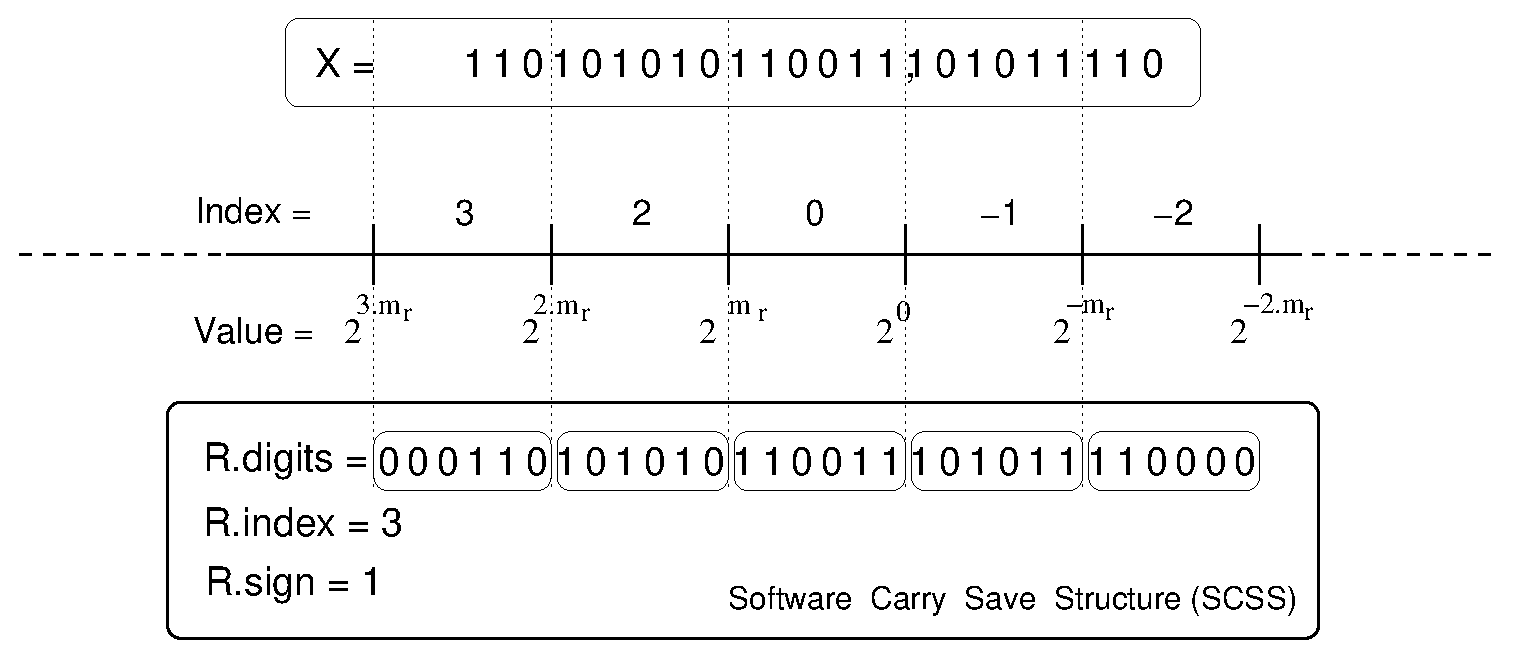
\includegraphics[width=0.7\textwidth]{fig_scs/exponent_representation} % image file name
\caption{The proposed format \label{fig:scsrepresentation}}
\end{center}
\end{figure}
  
In other words, the value  $x$ of a representation $R$  is:
\begin{equation}
\label{eqn4}
x = R.sign \times \sum_{j=1}^{n_r} R.digits[j] \times 2^{m_r * (R.index - j)}
\end{equation}

In such a \emph{normal} SCS number $R$, the bits from $m_I$ to $m_r$
of the $R.digits$ fields are thus set to zero. They will be exploited
by the algorithms to store temporary \emph{carry} information, and are
therefore called \emph{carry-save} bits. An SCS number where these
bits are non-zero is said to be non-normal.

The values of the parameters for use in \crlibm\ is $n_r=8$ digits of
$m_i=30$ bits stored on $m_r=32$-bit words. The worst-case precision
that this format may hold is when the most significant digit is equal
to $1$, meaning that an SCS numbers holds only $1+7\times 30=211$
significant digits.


\subsection{Arithmetic operations\label{sec:ops}}


\subsubsection{Conversion from double to SCS}
 A first method for converting a double precision floating
point number $d$ into an SCS representation is to extract the
exponent $d_{exp}$ from $d$, and then determine the corresponding
$R.index$ as the integer part of
$\frac{d_{exp}}{2^{m_r}}$.

Another method uses a variable number of multiplications by
$2^{m_r}$ or $2^{-m_r}$. This method is faster than the previous one
when the exponent of $d$ is close to $0$.

After testing both methods in \crlibm, the first method was preferred.


\subsubsection{Addition and subtraction}

The addition of two SCS numbers of the same sign consists in aligning,
then adding digits of the same order. Thanks to the carry-save bits,
all these additions will be \emph{exact} and \emph{independent}.
However the result will usually not be a normal SCS number: the sums
will have overflown in the carry-save bits. A \emph{renormalization}
procedure is presented in section \ref{renorm} to propagate these
carry bits and get again a normal SCS number.  However, the advantage
of SCS representation is that many SCS numbers can be summed before
needing to perform this expensive step (up to 7 with the choice of
parameters made in \crlibm).

The subtraction (addition of two numbers of opposite signs) is very
similar to the addition algorithm. It may also classically lead to a
cancellation, which may need an update of the index of the result.
However, as in other floating-point formats, a subtraction involving a
a cancellation is exact.

Although all the digit operations are exact, the addition or
subtraction of two numbers also classically involves a rounding error,
due to aligning the digits of same magnitude. For performance reason
this rounding is a truncation, so the worst-case relative error is one
ulp of the least accurate representable number, or $2^{-211}$.




%---------------- 
% MULTIPLICATION
%----------------
\subsubsection{Multiplication}

The multiplication of two normal SCS numbers involves the operations
depicted on the Figure \ref{fig:scsmultiplication}: The partial
products are computed (in parallel) and summed in columns. The
parameters are set up so that none of these operation overflow. Again,
the result is not a normal SCS number, and a renormalization procedure
(described below) has to be applied to empty the carry bits. However,
a few additions may follow a multiplication before this
renormalization, which allows for further optimization of algorithms
using SCS arithmetic. For instance, a polynomial evaluation can be
implemented with a renormalization after one multiplication and one
addition.

\begin{figure}[h]
\begin{center}
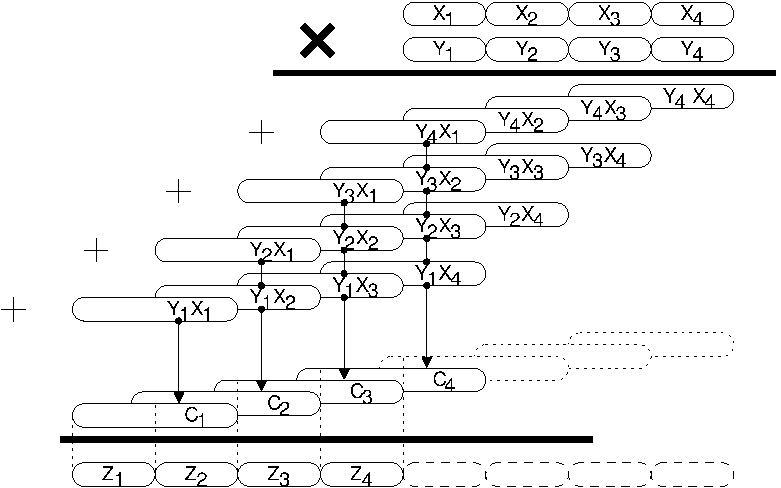
\includegraphics[width=0.7\textwidth]{fig_scs/multiplication}
\caption{SCS multiplication \label{fig:scsmultiplication}}
\end{center}
\end{figure}

Here also, a rounding error is involved when two $n_r$-digit numbers
are multiplied if the result is to fit on $n_r$ digits. The actual
implementation tests if the most significant digit ($z_1$ on
Figure~\ref{fig:scsmultiplication}) is null, in which case the index of
the result is that of $z_2$.

If the whole of the computations of
Figure~\ref{fig:scsmultiplication} are implemented, the worst case
for relative accuracy is again $2^{-211}$. However a further
optimization is to avoid computing the columns of lower magnitude, at
the expense of an increase in the rounding error. More specifically,
we compute 9 columns instead of 16.  The wors case is now when $z_1$
is null, in which case the relative error correspond to the truncation
of the 8 leftmost columns, whose maximum value is smaller than 3 ulps
of the SCS result. Therefore the relative error of the multiplication
is bounded by $2^{-208}$ with this optimization, which is still a
large overkill for the purpose of \crlibm.

This optimization is therefore implemented if the loop are hand-unrolled.
If they are not, the increased control complexity actually degrades
performance.


\subsubsection{Renormalization (carry propagation) \label{renorm}}

Renormalization is a carry propagation from the low order to high
order digits: Starting with an initially null carry, at each step, the
previous carry is added to the current digit, and this sum is then
split into two parts using masks. The low $m_r$ bits are a digit of
the normalized result, and the upper part is the next carry.

The actual algorithm is a little bit more complex. The initial
non-normal number may not be representable exactly as a normal SCS
number, therefore the index of the normalized result may have to be
increased by one or two.  Normalization thus again involves a rounding
error. Note that this error was already taken into account in the previous
discussions of addition and multiplication.




%-----------------
% CONVERSION BACK
%-----------------
\subsubsection{Conversion from SCS to floating-point}

A few (4 in the worst case) multiplications and additions suffice to
get the FP number closest to a SCS number.  For instance, for $m_I=53$
and $m_r=26$, we need to compute $d = A.sign \times 2^{A.index \times
  m_r} \times ( A.digits[0]+ 2^{-m_r} \times A.digits[1]+ 2^{-2.m_r}
\times A.digits[2]+ 2^{-3.m_r} \times A.digits[3])$. The number
$2^{A.index \times m_r}$ is build using integer masks. The actual
implementation of this formula is slightly less simple, but this
conversion is still very fast.


\subsubsection{Mixed 32- and 64-bit arithmetics}

An improvement implemented in \scslib\ was the combined use of integer 32- and 64-bit
arithmetics as follows: 

\begin{itemize}
\item MP digits are stored as 32-bit numbers where only a few bits are
  reserved for carries. This removes the main problem of the initial
implementation \cite{DefDin2002}, namely its memory inefficiency.

\item Addition uses 32-bit arithmetic. 

\item In the MP multiplication, the partial products are products of
  two 32-bit digits, which are 64-bit numbers. The column sums need
  thus to be computed using 64-bit arithmetic. This can be expressed
  in the C language in a non-ANSI-C99, but de-facto standard way, as
  follows: 32-bit numbers have the \texttt{unsigned int} type; 64-bit
  numbers have the \texttt{unsigned long long int} type. When
  multiplying two digits, one is first cast into this 64-bit type.
  
  For UltraSPARC architectures (detected at build time) the
  conversion is to floating-point, but we will not detail this
  peculiarity further.
\end{itemize}


This works well because all modern processors either have 64-bit
integer units, or offer instructions which store the 64-bit product of
two 32-bit integers into two 32-bit registers. The compiler does the
rest well, because it is conceptually simple: casting unsigned 32-bit
into unsigned 64-bit is trivial; 64-bit addition is translated
straightforwardly into one 32-bit \emph{add} followed by one 32-bit
\emph{add-with carry}.




\subsubsection{Implementation considerations}

For portability purposes, the implemention uses ANSI C as defined by
the C99 standard, and tries to use a recent version of \texttt{gcc}.
We could not exhibit a case where a native compiler from the processor
vendor (Intel or Sun) gave significantly better results than
\texttt{gcc}, which is probably a consequence of the simplicity of our
code.

However, when tuning for performance, we observed that the same code
which was efficient on one processor could lead to very poor results
on another.  Usually, this difference can be traced down to the
capabilities of the processor itself. The typical example is the
knowingly poor integer multiplication on UltraSPARC II. Sometimes
however, the processor should be able to perform well, and it is the
processor-specific backend of the compiler which is to blame, which
can be checked by observing the assembly code produced.  A typical
example is the casting of 32-bits digits to 64-bit arithmetic (or to
an FP number in the case of the UltraSPARC) in the multiplication
algorithm. In these cases we tried to change the programming style in
a way that works well on all processors. Sometimes it wasn't possible,
in which case the code contains, along with a generic version, several
processor-specific tricky versions of the problematic operation,
selected at compile time thanks to the GNU \texttt{automake/autoconf}
tools.


More surprisingly, we were disappointed by the higher-level
capabilities of the compilers, especially at unrolling loops. Our code
exhibits many small \texttt{for} loops whose size is known at
compile-time (usually $n$). This is the ideal situation for loop
unrolling, a technique well known and described in most textbooks on
compiler design. Options exist in most compilers to turn on this
optimisation. Unfortunately, leaving loop unrolling to the compiler
gives very poor results, even when compared to the non-unrolled case.
Since unrolling the loops by hand in the C code takes a few minutes,
we did it for the version of the library which we use ($m=30$, $n=8$).
It marginally increases the code sizes for this small $n$, and
sometimes provides a twofold improvement on speed, depending of the
processor. Of course, this is not satisfactory: We don't want to do it
for all values of $n$, nor do we want to study for each processor the
tradeoffs involved as $n$ increase. We expect however future compilers
to handle unrolling better, and we were surprised that no compiler had
a clear edge on the other in this respect. Some argue, however, that
this issue is pointless, as superscalarity, along with register
renaming and branch prediction inside modern processors, sum up to the
equivalent of dynamic unrolling of the code. In our tests (in 2003), it
doesn't: unrolling does bring a speed-up.








\section{Common Maple procedures \label{section:commonMaple}}


\subsection{Conversions}





Procedure \texttt{ieeedouble} returns the sign, the exponent and the
mantissa of the IEEE-754 double-precision number closest to input
value \texttt{x}.

\begin{lstlisting}[caption={ieeedouble},firstnumber=1]
ieeedouble:=proc(xx)
local x, sgn, logabsx, exponent, mantissa, infmantissa,powermin,powermax,expmin,expmax,expmiddle,powermiddle;
Digits := 100;
x := evalf(xx);
if (x=0) then sgn, exponent, mantissa := 1, -1022, 0
else
  if (x < 0) then sgn := -1
  else sgn := 1
  fi:
  x := abs(x);
  if x >=  2^(1023)*(2-2^(-53)) then mantissa := infinity; exponent := 1023
  else if x <= 2^(-1075) then mantissa := 0; exponent := -1022
      else
         if x <= 2^(-1022) then exponent := -1022
         else
# x is between 2^(-1022) and 2^(1024)
         powermin := 2^(-1022); expmin := -1022;
         powermax := 2^1024; expmax := 1024;
         while (expmax-expmin > 1) do
            expmiddle := round((expmax+expmin)/2);
            powermiddle := 2^expmiddle;
            if x >= powermiddle then
                powermin := powermiddle;
                expmin := expmiddle
            else
                powermax := powermiddle;
                expmax := expmiddle
            fi
          od;
# now, expmax - expmin = 1 and powermin <= x < powermax,
# powermin = 2^expmin and powermax = 2^expmax, so expmin is the exponent of x
         exponent := expmin;
         fi;
         infmantissa := x*2^(52-exponent);
	 if frac(infmantissa) <> 0.5 then mantissa := round(infmantissa)
            else
              mantissa := floor(infmantissa);
               if type(mantissa,odd) then mantissa := mantissa+1 fi
            fi;
         mantissa := mantissa*2^(-52);
      fi;
  fi;
fi;
sgn,exponent,mantissa;
end:
\end{lstlisting}


Procedure \texttt{ieeehexa} returns the hexadecimal representation of the nearest double to its input \texttt{x}.

\begin{lstlisting}[caption={ieeehexa},firstnumber=1]
ieeehexa:= proc(x)
local  hex2, xx, longint, expo, sgn, frac, resultat;
    if(x=0) then resultat:=["00000000","00000000"];
    elif(x=-0) then resultat:=["80000000","00000000"]; # nice try
    else
        xx:=ieeedouble(x);
        sgn:=xx[1]:
        expo:=xx[2]:
        frac:=xx[3]:
        if (expo = -1023) then
            longint := (frac)*2^51 ;   # subnormal
        else
            longint := (frac-1)*2^52 +   (expo+1023)*2^52;
        fi:
        if (sgn=-1) then
            longint := longint + 2^63;
        fi:
        longint := longint + 2^64:  # to get all the hexadecimal digits when we'll convert to string
        hex2:=convert(longint, hex);
        hex2:=convert(hex2, string):

        resultat:=[substring(hex2,2..9), substring(hex2,10..18)]:
    fi:
    resultat;
end proc:
\end{lstlisting}

Procedure \texttt{hexa2ieee} performs the reciprocal conversion.





Procedure \texttt{hi\_lo} returns two IEEE-double numbers $x\_hi$ and
$x\_lo$ so that $x = x\_hi + x\_lo + \epsilon_{-103}$.

\begin{lstlisting}[caption={hi\_lo},firstnumber=1]
hi_lo:= proc(x)
local x_hi, x_lo, res:
x_hi:= nearest(evalf(x)):
res:=x-x_hi:
if (res = 0) then
  x_lo:=0:
else
  x_lo:=nearest(evalf(res)):
end if;
x_hi,x_lo;
end:
\end{lstlisting}
\vspace{0.5cm}




Procedure \texttt{showHowDifficultToRound} takes a real number, and prints
the bits after the 53th of its nearest IEEE floating-point number.


\begin{lstlisting}[caption={showHowDifficultToRound},firstnumber=1]
showHowDifficultToRound:=proc(x)
local xb,xs,s,e,m:
    Digits:=200:
    s,e,m := ieeedouble(x):
    xb:=convert(evalf(x*2^(-e)),binary):
    xs:=convert(xb, string):
    substring(xs,55..153)
end proc:
\end{lstlisting}


\subsection{Procedures for polynomial approximation}


Procedure \texttt{Poly\_exact2} takes in arguments a polynomial
\texttt{P} and a integer \texttt{n}. It returns a truncated
polynomial, of which coefficients are exactly IEEE-double numbers. The
\texttt{n} first coefficients are written over 2 IEEE-double numbers.

\begin{lstlisting}[caption={poly\_exact2},firstnumber=1]
poly_exact2:=proc(P,n)
local deg,i, coef, coef_hi, coef_lo, Q:
Q:= 0:
convert(Q, polynom):
deg:=degree(P,x):
  for i from 0 to deg do
    coef :=coeff(P,x,i):
    coef_hi, coef_lo:=hi_lo(coef):
    Q:= Q + coef_hi*x^i:
    if(i<n) then
        Q := Q + coef_lo*x^i:
    fi:
  od:
  return(Q);
end:
\end{lstlisting}
\vspace{0.5cm}


We also have procedures for computing good truncated polynomial
approximation for a function. As they are useless to the proof, we do
not describe them here, the interested reader is referred to file
\texttt{maple/common-procedures.mpl} for more details.










\subsection{Accumulated rounding error in Horner evaluation
 \label{sec:Horner-maple}}



The following Maple procedures implement the error analysis described
in Section~\ref{sec:Horner}.

Procedure \texttt{compute\_abs\_rounding\_error} computes a bound on
the accumulated rounding error caused by the Horner evaluation of a
truncated polynomial. \texttt{poly} is the polynomial, \texttt{xmax} is the max value of
$|x|$, \texttt{nn} is the degree when \texttt{poly} is computed in double double, and the
first double-double operation is an addition.

This procedure returns the maximum absolute error, and safe bounds on the
minimum and maximum values of the function. It also checks on the fly
that the fast (test-free) versions of the double-double addition can
be used, and prints warnings if it not the case.

\begin{lstlisting}[caption={compute\_abs\_rounding\_error},firstnumber=1]
compute_abs_rounding_error:=proc(poly,xmax, nn)
local n, deg, delta, deltap, i, S, P, Snorm, Smin, Smax, prec:
deltap:=0:
delta:=0:
deg:=degree(poly):

prec:=53; # precision of the first iterations

S:=coeff(poly, x, deg):
Smax:=abs(S):
Smin:=Smax:

if nn<0 then n:=0: else n:=nn: fi:# sometimes called by compute_rel_rounding_error with n=-1

for i from (deg-1) to 0 by -1 do
  P:= convert(S*x, polynom):
  Smin := abs(coeff(poly,x,i)) - xmax*Smax : 
  if(Smin<=0) then 
    printf("Warning! in compute_abs_rounding_error, Smin<=0 at iteration %d, consider decreasing xmax\n",i);
  fi:
  delta:= evalf(xmax*deltap + 2**(-prec)*xmax*Smax):
  if i<n then 
    # fast Add22 ?    
    if abs(coeff(poly,x,i)) < xmax*Smax  # may be improved to xmax*Smax/2
    then printf("WARNING Add22 cannot be used at step %d, use Add22Cond\n" , i  );   
         printf("    coeff=%1.20e,  xmax*Smax=%1.20e"  ,  abs(coeff(poly,x,i)),  xmax*Smax );
    fi:
  fi:
  S:=convert(P+coeff(poly,x,i), polynom):
  Snorm:=evalf(infnorm(S, x=-xmax..xmax)):
  if i=n-1 then prec:=100: fi:  # from the addition of the n-1-th iteration
  deltap:= evalf(delta + 2**(-prec)*(delta + Snorm)): 
  Smax := Snorm + deltap:  
od:
deltap, Smin, Smax;
end proc:
\end{lstlisting}
\vspace{0.5cm}

Procedure \texttt{compute\_rel\_rounding\_error} computes a bound on
the total relative rounding error of a Horner polynomial evaluation,
in the same condition as the previous procedure.

\begin{lstlisting}[caption={compute\_abs\_rounding\_error},firstnumber=1]
compute_rel_rounding_error:=proc(poly,xmax, n)
local deg, p, rho, deltap, Smin, Smax:

deg:=degree(poly):
if(n>0) then p:=100: else p:=53: fi: 

if coeff(poly,x, 0) = 0 then
   deltap, Smin, Smax := compute_abs_rounding_error(poly/x,xmax, n-1):
   rho :=  (2^(-p)*(Smax+deltap) +deltap ) / Smin :
else
   deltap, Smin, Smax := compute_abs_rounding_error(poly,xmax, n):
   rho := deltap /  Smin:
fi:
rho;
end proc:
\end{lstlisting}
\vspace{0.5cm}

Procedures \texttt{compute\_abs\_rounding\_error\_firstmult} and
\texttt{compute\_abs\_rounding\_error\_firstmult} are similar to the
previous, but in the case when the first double-double operation is a
multiplication.



\subsection{Rounding}

Procedure \texttt{compute\_rn\_constant} computes the best (smallest)
possible constant for the round-to-nearest test of
Theorem~\ref{th:roundingRN1}, for an input delta which is the overall
relative error of the approximation scheme

\begin{lstlisting}[caption={compute\_rn\_constant},firstnumber=1]
compute_rn_constant := proc(delta)
  local k;
  k := trunc(-log2(delta)) - 53: 
  nearest(  1+ 2**(-52) + (2**(54+k)*delta)  /  ( (2**k-1) * (1-2**(-53)) )  ):
end proc:
\end{lstlisting}
\vspace{0.5cm}



\subsection{Using double-extended}

The file \texttt{maple/double-extended.mpl} contains procedures
similar to those previously described to handle double-extended
precision (64 bits of mantissa and 15 bits of exponent). This is
currently used in experimental code only: The \crlibm\ CVS repository
at \url{http://lipforge.ens-lyon.fr/} contains such code for
exponential and arctangent on Itanium, and arctangent on IA32
processors. For more details see \cite{DinDefLau2004LIP,DinGast2005}.
